\documentclass[11pt,a4paper]{article}
\usepackage{amsmath}
\usepackage{amssymb}
\usepackage{graphicx}
\usepackage{verbatim}
\begin{document}
\noindent
Martin Lundfall, Henri Bunting, Malte Siemers, Patrik Bey
\begin{centering}
  \section*{Exercise sheet 08 - Machine Intelligence I}
  \end{centering}
\section*{8.1}
Given:
\begin{equation}
C_{(p, N)} = 2*\sum_{k = 0}^{N - 1}{p-1 \choose k}
\end{equation}
Prove:
\begin{equation}
C_{(p, N)} + C_{(p, N-1)} = C_{(p+1, N)}
\end{equation}
Proof:\\
By the definition of C, we can rewrite into sums:
\begin{equation}
2*\sum_{k = 0}^{N - 1}{p-1 \choose k} + 2*\sum_{k = 0}^{N - 2}{p-1 \choose k} = 2*\sum_{k = 0}^{N - 1}{p \choose k}
\end{equation}
We can then divide out the 2:
\begin{equation}
\sum_{k = 0}^{N - 1}{p-1 \choose k} + \sum_{k = 0}^{N - 2}{p-1 \choose k} = \sum_{k = 0}^{N - 1}{p \choose k}
\end{equation}
We know:
\begin{equation}
\sum_{k = 0}^{0}{p-1 \choose k} = {p-1 \choose 0} = 1
\end{equation}
So we pull out the first k=0 terms:
\begin{equation}
1+\sum_{k = 1}^{N - 1}{p-1 \choose k} + \sum_{k = 0}^{N - 2}{p-1 \choose k} = 1+\sum_{k = 1}^{N - 1}{p \choose k}
\end{equation}
But then we subtract them to get rid of them and rewrite the second term so that k starts at 1:
\begin{equation}
\sum_{k = 1}^{N - 1}{p-1 \choose k} + \sum_{k = 1}^{N - 1}{p-1 \choose k-1} = \sum_{k = 1}^{N - 1}{p \choose k}
\end{equation}
Since the sums have the same indices, we can reform them into a single sum:
\begin{equation}
\sum_{k = 1}^{N - 1}({p-1 \choose k} + {p-1 \choose k-1}) = \sum_{k = 1}^{N - 1}{p \choose k}
\end{equation}
And after dropping the sums we get:
\begin{equation}
{p-1 \choose k} + {p-1 \choose k-1} = {p \choose k}
\end{equation}

Which is the same as the binomial theorem:
\begin{equation}
{r \choose q} + {r \choose q-1} = {r+1 \choose q}
\end{equation}

\section*{8.2}
\subsection*{a)}

\begin{figure}[h]
  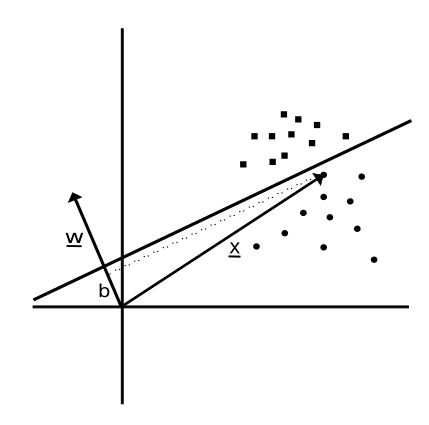
\includegraphics[width=0.8\textwidth]{geometry.png}
  \caption{Geometry of a linear classifier. $\underline{\mathbf{x}}$ is the vector to the location of a data point, $\underline{\mathbf{w}}$ the weight vector of the neuron and $\mathbf{b}$ the distance from the origin to the classification boundary.}
\end{figure}

The geometry of a binary classifier of form $y = sign(\underline{\mathbf{w}}^T\underline{\mathbf{x}} - b)$ is illustrated above. The decision boundary is orthogonal to the weight vector $\underline{\mathbf{w}}$ with distance b to the origin. $\underline{\mathbf{w}}^T\underline{\mathbf{x}}$ is the projection of $\underline{\mathbf{x}}$ on $\underline{\mathbf{w}}$ and b shifts the decision boundary according to the classification problem, so that $sign(\underline{\mathbf{w}}^T\underline{\mathbf{x}} - b)$ becomes negative for points on one side of the boundary and positive for the other.

\subsection*{b)}



\section*{8.3}
\subsection*{a)}
A margin can be thought of as the 'width' of the decision boundary of the linear connectionist neuron, or how close we allow the boundary line to come to the data points. The effect of increasing the margin is that the number of possible classifying lines decreases which effectively reduces the complexity of the classifier. If this can be done without affecting the training/empirical error of the classifier, it can reduce the generalization error.
\subsection*{b)}
The Euclidean distance $d(x^\alpha,w,b)$ from a sample $x^{(\alpha)}$ to the decision boundary line $L = \{ x \in X | w^Tx + b = 0\}$ is given by 
\begin{equation}
d(x^\alpha,w,b) = |\frac{w^Tx^{(\alpha)}}{||w||}+\frac{- b}{||w||}| = \frac{1}{||w||}\left ( w^Tx^{(\alpha)} + b \right )
\end{equation}
With the constraint that $w^Tx^{(\alpha)} + b \leq 1$ for all $x \in X$, we get 
\begin{equation}
d(x^\alpha,w,b) \leq \frac{1}{||w||}
\end{equation}
\subsection*{c)}
The \textit{primal optimization problem} offers a method of maximizing the margin of the classifier while keeping the constraint that we still classify all training points correctly. This is done by using the Kuhn–Tucker conditions, a generalization of Lagrange multipliers, which involves minimizing the Lagrange equation:
\begin{equation}
  L_{(x_k, \{\lambda_k\})} = f_0(x) + \sum_{k=1}^m \lambda_k f_k(x)
\end{equation}
Where $f_k$ are constraints expressed in the form that they must be smaller than or equal to zero, and $f_0(x)$ is the function that we want to minimize. In our case, the constraint set by normalizing the margin gives $f(x) = -(y_T(w^Tx + b) -1)$ on this form. Since we want to maximize the margin, we want to minimize $f_0(x) = \frac{||w||^2}{2}$.\\
The aim is to minimize the Lagrangian function, and we do this by first minimizing with respect to $w$. This will result us an expression on the form:
\begin{equation}
w = \sum_{\alpha=1}^p \lambda_\alpha y_T^{(\alpha)}x^{(\alpha)}
\end{equation}
Where $\alpha$ is indexing over $p$ datapoints. Then, minimizing with respect to $b$ we get the following constraint on $\lambda$ and $y_T$:
\begin{equation}
0 = - \sum_{\alpha=1}^p \lambda_\alpha y_T^{(\alpha)}
\end{equation}
Putting these results back into the Lagrange equation, we attain:
\begin{equation}
L_{(x_k, \{\lambda_k\})} = -\frac{1}{2} \sum _{\alpha, \beta=1}^p\lambda_\alpha \lambda_\beta y_T^{(\alpha)}y_T^{(\beta)}(x^{(\alpha)})^Tx^{(\beta)}+\sum_{\alpha=1}^p\lambda_\alpha
\end{equation}
The Khuhn-Tucker conditions implies that $w$ can be given as a linear combination of the data points:
\begin{equation}
w = \sum_{\alpha}^p\lambda_\alpha y_T^{(\alpha)}x^{(\alpha)}
\end{equation}
and the $b$ can be given by looking at the support vectors, i. e. the points that lie closest to the decision boundary and therefore satisfy:
\begin{equation}
y_T^{(\alpha)}(w^Tx^{(\alpha)}+b) = 1
\end{equation}
And we get:
\begin{equation}
b = \frac{1}{N_{SV}}\sum_{i = 1} ^{N_{SV}}(w^Tx_i - y_i)
\end{equation}
Where $i$ is indexing over the number of support vectors, $N_{SV}$.
\section*{8.4}
\subsection{a)}
Since we have that the support vectors, i.e. the datapoints lying closest to the decision boundary satisfy $y_T^{(\alpha)}(w^Tx^{(\alpha)}+b) = 1$, the remaining datapoints will require $\lambda$ to be zero in order to minimize the lagrangian. Therefore, it turns out that these are the only vectors we really have to pay attention to, and the others are already 'decided' by classifying with respect to the support vectors.
\subsection{b)}
In Exercise 8.3, we derived the following conditions:
\begin{equation}
w = \sum_{\alpha=1}^p \lambda_\alpha y_T^{(\alpha)}x^{(\alpha)}
\end{equation}
\begin{equation}
0 = - \sum_{\alpha=1}^p \lambda_\alpha y_T^{(\alpha)}
\end{equation}
We put this into the Lagrangian:
\begin{equation}
\begin{split}
L_{(x_k, \{\lambda_k\})} =  \frac{1}{2} \sum _{\alpha, \beta=1}^p\lambda_\alpha \lambda_\beta y_T^{(\alpha)}y_T^{(\beta)}(x^{(\alpha)})^Tx^{(\beta)}-
\\\sum _{\alpha=1}^p\lambda_\alpha y_T^{(\alpha)} \left (\sum_{\beta=1}^p \lambda_\beta y_T^{(\beta)}(x^{(\beta)})^T \right ) x^{(\alpha)}  -\sum_{\alpha=1}^p\lambda_\alpha y_T^{(\alpha)}- \sum_{\alpha=1}^p\lambda_\alpha
\end{split}
\end{equation}
The penultimate term term will disappear thanks to the constraint given by optimizing wwith respect to $b$, and we see that the first two terms are the same except for the constant, and we arrive at the given expression.
\section*{8.5}
\end{document}

^ ^

^
^
^
^
